\chapter{Potentials}

\section{Functional forms of force fields}

The molecular energy can be described as an Taylor expansion in bonds, bends, torsions, etc.
\begin{equation}
 \begin{split}
 U=&\sum_{\text{bonds}} U_r\left(r\right)+\sum_{\text{bends}} U_\theta\left(\theta\right)+
   \sum_{\text{torsions}} U_\phi\left(\phi\right)+\sum_{\text{out-of-plane bends}} U_\chi\left(\chi\right)
   +\sum_{\text{non-bonded}}U_{nb}\left(r\right)\\
   &+\sum_{\text{bond-bond}}U_{bb'}\left(r,r'\right)
   +\sum_{\text{bond-bend}}U_{b\theta'}\left(r,\theta\right)
   +\sum_{\text{bend-bend}}U_{\theta\theta'}\left(\theta,\theta'\right)\\
   &+\sum_{\text{bond-torsion}}U_{r\phi}\left(r,\phi,r'\right)
   +\sum_{\text{bend-torsion}}U_{\theta\phi}\left(\theta,\phi,\theta'\right)+\dots
  \end{split}
  \label{Eq: force field}
\end{equation}
This expansion is believed to capture all the chemical entities we can think of, such as
atoms, bonds, angles, etc, and physical properties like equilibrium structures, vibrational spectra, etc.
The cross terms are not ad-hoc functions, but arise naturally from this expansion. 
For example, bonds and bends interact, as the bend angle becomes smaller the bond lengths tend to increase.
Their inclusion leads to two advantages: 1) they increase the accuracy of the force field
(especially the vibrational frequencies), and 2) they
increase the transferability of the diagonal terms $U_r\left(r\right),U_\theta\left(\theta\right),
U_\phi\left(\phi\right),U_\chi\left(\chi\right)$.
On top of the terms in Eq. \ref{Eq: force field} one can add ad hoc terms, such as hydrogen bonding, that
are not adequately accounted for otherwise.

Eq. \ref{Eq: force field} is historically referred to as an \emph{force field}. The name arose from the lowest
order approximation using only springs with \emph{force constants}. Force fields have matured
and have become quite accurate and many parameters exists for a wide range of structure. These parameters
are crucial and determine the quality of the force field. Unfortunately, deriving high quality parameters
remains more than a art rather than a science. However, some progress has been made and in the end of the chapter
some algorithms are described how to obtain them.

The terms in Eq. \ref{Eq: force field} consists of a functional form, force constants
(a resistance against a change from the optimum value), and a reference value.
The functional form is chosen such as to be an accurate description of the true potential energy (either
known from experiment or from quantum mechanics), although one can simplify the functional form to decrease
computational evaluation time of the energy at the cost of diminished accuracy. This tradeoff has almost vanished
for intra-molecular potentials but is still an issue for the non-bonded terms.
The reference value is \emph{not} the equilibrium value (except by chance).
For example, bond lengths are affected by all other terms in the force field and the more strained a molecule
the farther the bond equilibrium length will deviate from its reference value. This means that one can not simply
take the equilibrium values from known experiment.

\section{Bonded potentials diagonal terms}

\subsection{Bond-stretching potentials}

The bond stretching potential describes the change in energy as the bond stretches and contracts.
The simplest functional form would be Hook's law:
\begin{equation}
  U=\frac{1}{2} k \left(r-r_0\right)^2
\end{equation}
where $k$ is the force constant and $r_0$ the reference value for the bond. This form is computationally
very fast, but not very realistic. It is well known that it is easier to stretch a bond than it is to
compress a bond. The `Morse' potential is an-harmonic and provides a much better description of the energy
\begin{equation}
  U= D\left(1-e^{-\alpha\left(r-r_0\right)}\right)^2
\end{equation}
Expanding around the equilibrium value leads to
\begin{equation}
 U=D\alpha^2\left(r-r_0\right)^2\left[1-\alpha\left(r-r_0\right)+\frac{7}{12}\alpha^2\left(r-r_0\right)^2\dots\right]
\end{equation}
The first terms is the harmonic potential (with $k=2D\alpha^2$) and for organic structures where distortions
from equilibrium are small the difference between the potentials are small. However, for larger deviations
the Morse potential provides a significantly better description.
The Morse potential provides a restoring force which goes to zero at long distances. For minimizations
starting far equilibrium could result in non-convergence. Some force fields solved this problem by
using modification of Hook's law. MM2 added a cubic term making the bond an-harmonic. However, this leads to large
negative energies for poor initial geometries with large distortions. MM3 added the quartic term to solve this.
Note the $7/12$ terms in the MM2/3 functional forms originate from the Taylor expansion of the Morse potential,
and the cubic and quartic terms are chosen to mimic the Morse potentials for moderate distortions.
Dinur and Hagler proposed a functional form based on inverse bond lengths which follows the true potential energy
compared to QM over an even wider range
\begin{equation}
 U=U_0+C_2\left(\frac{1}{r}-\frac{1}{r_0}\right)^2+C_3\left(\frac{1}{r}-\frac{1}{r_0}\right)^3
\end{equation}

\noindent
The implemented bond-potentials:
\begin{itemize}

  \item{HARMONIC\_BOND}
  \begin{equation}
  U=\frac{1}{2} p_0 \left(r-p_1\right)^2
  \end{equation}
  2 arguments: $p_0/k_B$ in units of K/\AA$^2$, $p_1$ in \AA.

  \item{CORE\_SHELL\_SPRING}
  \begin{equation}
  U=\frac{1}{2} p_0 r^2
  \end{equation}
  1 argument: $p_0/k_B$ in units of K/\AA$^2$.

  \item{MORSE\_BOND}
  \begin{equation}
  U=p_0\left[\left(1-e^{-p_1\left(r-p_2\right)}\right)^2-1\right]
  \end{equation}
  3 arguments: $p_0/k_B$ in units of K, $p_1$ in \AA$^{-1}$, and $p_2$ in \AA.

  \item{LJ\_12\_6\_BOND}
  \begin{equation}
  U=\frac{p_0}{r^{12}}-\frac{p_1}{r^{6}}
  \end{equation}
  2 arguments: $p_0/k_B$ in units of K\,\AA$^{12}$, and $p_1/k_B$ in units of K\,\AA$^6$.

  \item{LENNARD\_JONES\_BOND}
  \begin{equation}
  U=4 p_0 \left[\left(\frac{p_1}{r}\right)^{12}-\left(\frac{p_1}{r}\right)^{6}\right]
  \end{equation}
  2 arguments: $p_0/k_B$ in units of K, $p_1$ in \AA.

  \item{BUCKINGHAM\_BOND}
  \begin{equation}
  U=p_0 e^{-p_1 r}-\frac{p_2}{r^{6}}
  \end{equation}
  3 arguments: $p_0/k_B$ in units of K, $p_1$ in units of \AA$^{-1}$, and $p_2/k_B$ in K\,\AA$^6$.

  \item{RESTRAINED\_HARMONIC\_BOND}
  \begin{equation}
  U=\begin{cases}
      \frac{1}{2} p_0\left(r-p_1\right)^2 & \qquad \left|r-p_1\right|\leq p_2\\
      \frac{1}{2} p_0 p_2^2+p_0 p_2\left(\left|r-p_1\right|-p_2\right) & \qquad \left|r-p_1\right|> p_2
     \end{cases}
  \end{equation}
  3 arguments: $p_0/k_B$ in units of K/\AA$^2$, $p_1$ in \AA, and $p_2$ in \AA.

  \item{QUARTIC\_BOND}
  \begin{equation}
  U=\frac{1}{2} p_0 \left(r-p_1\right)^2+ \frac{1}{3} p_2 \left(r-p_1\right)^3+ \frac{1}{4} p_3 \left(r-p_1\right)^4
  \end{equation}
  4 arguments: $p_0/k_B$ in units of K/\AA$^2$, $p_1$ in \AA, $p_2/k_B$ in K/\AA$^3$, and $p_3/k_B$ in K/\AA$^4$.

  \item{CFF\_QUARTIC\_BOND}
  \begin{equation}
  U=p_0 \left(r-p_1\right)^2+ p_2 \left(r-p_1\right)^3+ p_3 \left(r-p_1\right)^4
  \end{equation}
  4 arguments: $p_0/k_B$ in units of K/\AA$^2$, $p_1$ in \AA, $p_2/k_B$ in K/\AA$^3$, and $p_3/k_B$ in K/\AA$^4$.

  \item{MM3\_BOND}
  \begin{equation}
  U=p_0 \left(r-p_1\right)^2\left(1-2.55\left(r-p_1\right)+\frac{7}{12}\,2.55^2\,\left(r-p_1\right)^2\right)
  \end{equation}
  2 arguments: $p_0$ in units of mdyne/\AA\, molecule, $p_1$ in \AA.

  \item{RIGID\_BOND}\\
  Use for connections between rigid units.

  \item{FIXED\_BOND}\\
  Use for bonds constraint using the `SHAKE' and `RATTLE'-algorithm. Applies to Monte-Carlo, Molecular Dynamics, and minimization.

  \item{MEASURE\_BOND}\\
  A histogram of the bond-distance can be computed.

\end{itemize}

\subsection{Urey-Bradley potentials}

The Urey-Bradley potential is sometimes used to account for the repulsion between two atoms bound to a common
atom. In more modern force field they are replaced by bond/bend cross potentials.
Urey-Bradley are essentially just bonds between 1-3 nearest neighbor atoms and 
the same range of potentials is offered as for 1-2 bonds in RASPA.


\begin{itemize}

  \item{HARMONIC\_UREYBRADLEY}
  \begin{equation}
  U=\frac{1}{2} p_0 \left(r-p_1\right)^2
  \end{equation}
  2 arguments: $p_0/k_B$ in units of K/\AA$^2$, $p_1$ in \AA.

  \item{MORSE\_UREYBRADLEY}
  \begin{equation}
  U=p_0\left[\left(1-e^{-p_1\left(r-p_2\right)}\right)^2-1\right]
  \end{equation}
  3 arguments: $p_0/k_B$ in units of K, $p_1$ in \AA$^{-1}$, and $p_2$ in \AA.

  \item{LJ\_12\_6\_UREYBRADLEY}
  \begin{equation}
  U=\frac{p_0}{r^{12}}-\frac{p_1}{r^{6}}
  \end{equation}
  2 arguments: $p_0/k_B$ in units of K\,\AA$^{12}$, and $p_1/k_B$ in units of K\,\AA$^6$.

  \item{LENNARD\_JONES\_UREYBRADLEY}
  \begin{equation}
  U=4 p_0 \left[\left(\frac{p_1}{r}\right)^{12}-\left(\frac{p_1}{r}\right)^{6}\right]
  \end{equation}
  2 arguments: $p_0/k_B$ in units of K, $p_1$ in \AA.

  \item{BUCKINGHAM\_UREYBRADLEY}
  \begin{equation}
  U=p_0 e^{-p_1 r}-\frac{p_2}{r^{6}}
  \end{equation}
  3 arguments: $p_0/k_B$ in units of K, $p_1$ in units of \AA$^{-1}$, and $p_2/k_B$ in K\,\AA$^6$.

  \item{RESTRAINED\_HARMONIC\_UREYBRADLEY}
  \begin{equation}
  U=\begin{cases}
      \frac{1}{2} p_0\left(r-p_1\right)^2 & \qquad \left|r-p_1\right|\leq p_2\\
      \frac{1}{2} p_0 p_2^2+p_0 p_2\left(\left|r-p_1\right|-p_2\right) & \qquad \left|r-p_1\right|> p_2
     \end{cases}
  \end{equation}
  3 arguments: $p_0/k_B$ in units of K/\AA$^2$, $p_1$ in \AA, and $p_2$ in \AA.

  \item{QUARTIC\_UREYBRADLEY}
  \begin{equation}
  U=\frac{1}{2} p_0 \left(r-p_1\right)^2+ \frac{1}{3} p_2 \left(r-p_1\right)^3+ \frac{1}{4} p_3 \left(r-p_1\right)^4
  \end{equation}
  4 arguments: $p_0/k_B$ in units of K/\AA$^2$, $p_1$ in \AA, $p_2/k_B$ in K/\AA$^3$, and $p_3/k_B$ in K/\AA$^4$.

  \item{CFF\_QUARTIC\_UREYBRADLEY}
  \begin{equation}
  U=p_0 \left(r-p_1\right)^2+ p_2 \left(r-p_1\right)^3+ p_3 \left(r-p_1\right)^4
  \end{equation}
  4 arguments: $p_0/k_B$ in units of K/\AA$^2$, $p_1$ in \AA, $p_2/k_B$ in K/\AA$^3$, and $p_3/k_B$ in K/\AA$^4$.

  \item{MM3\_UREYBRADLEY}
  \begin{equation}
  U=p_0 \left(r-p_1\right)^2\left(1-2.55\left(r-p_1\right)+\frac{7}{12}\,2.55^2\,\left(r-p_1\right)^2\right)
  \end{equation}
  2 arguments: $p_0$ in units of mdyne/\AA\, molecule, $p_1$ in \AA.

 \item{RIGID\_UREYBRADLEY}\\
  Use for connections between rigid units.

  \item{FIXED\_UREYBRADLEY}\\
  Use for bonds constraint using the `SHAKE' and `RATTLE'-algorithm. Applies to Monte-Carlo, Molecular Dynamics, and minimization.

  \item{MEASURE\_UREYBRADLEY}\\
  A histogram of the Urey-Bradley distance can be computed.

\end{itemize}

\subsection{Bending potential}

The simplest approach for an angle potential is the harmonic potential
\begin{equation}
  U=\frac{1}{2} k \left(\theta-\theta_0\right)^2
\end{equation}
Angles are much softer than bonds, especially in zeolites where a Si-O-Si angle ranges 
between 135 and 180 degrees.
A problem with all polynomial representations of angles is that angles of 180 degrees results
in singular point (unless the reference angle is 180 degrees). The case of 0 degree is not possible
due to repulsion of the i and k atoms in the i-j-k bend.
The singularity is due to the fact that the force expression of such a polynomial
contains a factor $1/\sin\left(\theta\right)$. A common solution is to use a trigonometric function
\begin{equation}
  U=\frac{1}{2} k \left[\cos\left(\theta\right)-\cos\left(\theta_0\right)\right]^2
\end{equation}
Note that close to the maximum these potentials have no restoring force, but for small distortions this
is not a problem.
The MM force fields use higher order terms. A six power term was needed to describe the highly bent
bicyclo[1.1.1]pentane. Cubic terms and higher become desirable when the bending is more then 10-15 degrees.
MM3 angle bending has been divided into in-plane and out-of-plane bending for planar trigonal centers.

\begin{itemize}

  \item{HARMONIC\_BEND,CORE\_SHELL\_BEND}\\
  \begin{equation}
  U=\frac{1}{2}p_0\left(\theta_{ijk}-p_1\right)^2
  \end{equation}
  2 arguments: $p_0/k_B$ in units of K/rad$^2$ and $p_1$ in degrees.

  \item{QUARTIC\_BEND}
  \begin{equation}
  U=\frac{1}{2} p_0 \left(\theta_{ijk}-p_1\right)^2+
     \frac{1}{3} p_2 \left(\theta_{ijk}-p_1\right)^3+
     \frac{1}{4} p_3 \left(\theta_{ijk}-p_1\right)^4
  \end{equation}
  4 arguments: $p_0/k_B$ in units of K/rad$^2$, $p_1$ in degrees, $p_2/k_B$ in K/rad$^3$, and $p_3/k_B$ in K/rad$^4$.

  \item{CFF\_QUARTIC\_BEND}
  \begin{equation}
  U=p_0 \left(\theta_{ijk}-p_1\right)^2+
    p_2 \left(\theta_{ijk}-p_1\right)^3+
    p_3 \left(\theta_{ijk}-p_1\right)^4
  \end{equation}
  4 arguments: $p_0/k_B$ in units of K/rad$^2$, $p_1$ in degrees, $p_2/k_B$ in K/rad$^3$, and $p_3/k_B$ in K/rad$^4$.

  \item{HARMONIC\_COSINE\_BEND}\\
  \begin{equation}
  U=\frac{1}{2}p_0\left(\cos\theta_{ijk}-\cos p_1\right)^2
  \end{equation}
  2 arguments: $p_0/k_B$ in units of K and $p_1$ in degrees.

  \item{COSINE\_BEND}\\
  \begin{equation}
  U=p_0\left(1+\cos\left(p_1\theta_{ijk}-p_2\right)\right)
  \end{equation}
  3 arguments: $p_0/k_B$ in units of K, $p_1$ dimensionless, and $p_2$ in degrees.

  \item{MM3\_BEND}
  \begin{equation}
  \begin{split}
  U=\frac{1}{2}p_0 \left(\theta_{ijk}-p_1\right)^2\Bigl(1-0.014\left(\theta_{ijk}-p_1\right)+
   5.6\times10^{-5}\left(\theta_{ijk}-p_1\right)^2&-7\times10^{-7}\left(\theta_{ijk}-p_1\right)^3\\
   &+2.2\times10^{-8}\left(\theta_{ijk}-p_1\right)^4
   \Bigr)
  \end{split}
  \end{equation}
  2 arguments: $p_0$ in units of mdyne\,\AA/rad$^2$, $p_1$ in degrees.
  \item{MM3\_IN\_PLANE\_BEND}
  \begin{equation}
  \begin{split}
  U=\frac{1}{2}p_0 \left(\theta_{ijk}-p_1\right)^2\Bigl(1-0.014\left(\theta_{ijk}-p_1\right)+
   5.6\times10^{-5}\left(\theta_{ijk}-p_1\right)^2&-7\times10^{-7}\left(\theta_{ijk}-p_1\right)^3\\
   &+2.2\times10^{-8}\left(\theta_{ijk}-p_1\right)^4
   \Bigr)
  \end{split}
  \end{equation}
  2 arguments: $p_0$ in units of mdyne\,\AA/rad$^2$, $p_1$ in degrees. The bend is `in-plane' and only applicable to bends in a defined planar trigonal centers.
  The bend is dependend on the fourth atom of the trigonal center.

  \item{FIXED\_BEND}\\
   Use for bend-angle constraint using the `SHAKE' and `RATTLE'-algorithm. Applies to Molecular Dynamics and minimization.
   Does not work (yet) in Monte-Carlo.

  \item{MEASURE\_BEND}\\
  A histogram of the bend angle can be computed.

\end{itemize}

\subsection{Wilson inversion-bend potential}

\begin{figure}[t]
  \centering
  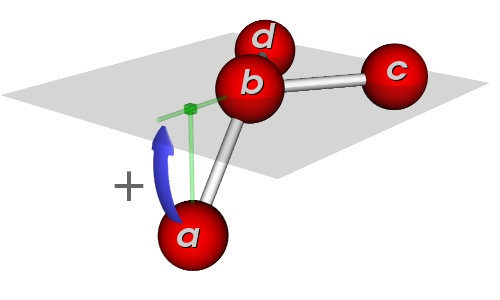
\includegraphics[width=7.5cm]{./Potentials/WilsonAnglePlus.jpg}
  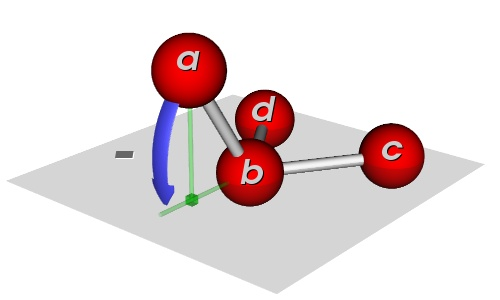
\includegraphics[width=7.5cm]{./Potentials/WilsonAngleMinus.jpg}
  \caption{The definition of the Wilson inversion-bend angle $\chi$.
  On the left a positive Wilson angle, and on the right a negative Wilson angle.}
  \label{Fig: Wilson definition}
\end{figure}

Common planar molecule that contain a double bond or sp$^2$ hybridization form planar groups with trigonal centers.
For example: the carbon and nitrogen centers in formamide, and the carbon centers in benzene.
The mode of motion is different from bond stretching, bending, and internal rotation.
The associated harmonic potential is
\begin{equation}
  U=\frac{1}{2} k \left(\chi\right)^2
\end{equation}
with $\chi$ the out-of-plane angle. Two possible definitions are in use
\begin{enumerate}
\item{the distance of the central atom from the plane defined by the other three atoms (pyramid height),}
\item{the average angle between any bond that extends from the central atom and the plane defined by the
other two bonds}.
\end{enumerate}
Note that an alternative to the out-of-plane angle is the \emph{improper torsion} using
\begin{equation}
  U=\frac{1}{2} k \left(1-\cos 2\chi\right)
\end{equation}
The out-of-plane potential can also be used for non-planar structure, for example in united-atom for chiral
centers to avoid inversion of the chiral center. Another example of its use is coordination complexes
where now the plane of the ligands need no longer be defined exactly.
In square planar complexes it is necessary to define an average plane through the ligands
(usually the least-square plane).
Note that the definition include one central atom
which is listed as the second in $a-b-c-d$: $a$, $c$, and $d$ are bonded to the central atom $b$.
The inversion angle potential is the average of the three possible inversion angle terms.

\begin{itemize}
  \item{HARMONIC\_INVERSION}\\
 \begin{equation}
  U=\frac{1}{2}p_0\left(\chi_{ijk}-p_1\right)^2
  \end{equation}
  2 arguments: $p_0/k_B$ in units of K/rad$^2$ and $p_1$ in degrees.
  \item{HARMONIC\_COSINE\_INVERSION}\\
 \begin{equation}
  U=\frac{1}{2}p_0\left(\cos\left(\chi_{ijk}\right)-\cos\left(p_1\right)\right)^2
  \end{equation}
  2 arguments: $p_0/k_B$ in units of K and $p_1$ in degrees.
  \item{PLANAR\_INVERSION}\\
 \begin{equation}
  U=p_0\left(1-\cos\left(\chi\right)\right)
  \end{equation}
  1 argument: $p_0/k_B$ in units of K.
  \item{MM3\_INVERSION}\\
  \begin{equation}
  \begin{split}
  U=\frac{1}{2}p_0 \left(\chi-p_1\right)^2\Bigl(1-0.014\left(\chi-p_1\right)+
   5.6\times10^{-5}\left(\chi-p_1\right)^2&-7\times10^{-7}\left(\chi-p_1\right)^3\\
   &+2.2\times10^{-8}\left(\chi-p_1\right)^4
   \Bigr)
  \end{split}
  \end{equation}
  2 arguments: $p_0$ in units of mdyne\,\AA/rad$^2$, $p_1$ in degrees.

  \item{FIXED\_INVERSION\_BEND}\\
   Use for inversion bend-angle constraint using the `SHAKE' and `RATTLE'-algorithm. 
   Applies to Molecular Dynamics and minimization. Does not work (yet) in Monte-Carlo.
\end{itemize}

\begin{figure}[t]
  \centering
  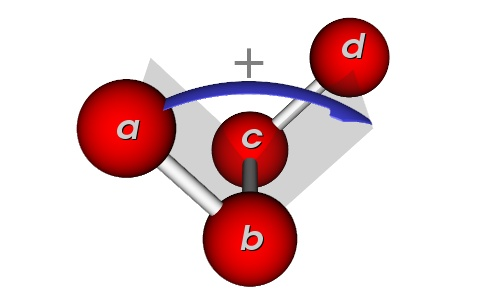
\includegraphics[width=7.5cm]{./Potentials/TorsionAnglePlus.jpg}
  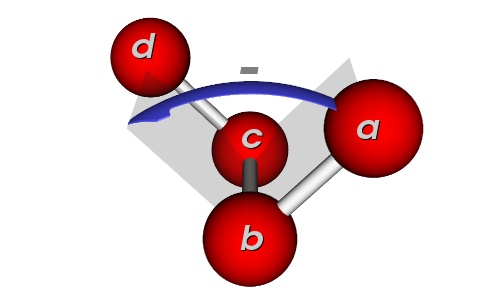
\includegraphics[width=7.5cm]{./Potentials/TorsionAngleMinus.jpg}
  \caption{The definition of the dihedral angle $\phi$: the angle between the planes formed by atoms a-b-c and b-c-d.
   On the left a positive dihedral angle, and on the right a negative dihedral angle.}
  \label{Fig: Torsion definition}
\end{figure}

\subsection{Torsion potential}

Intramolecular rotations about bonds do not occur freely. A possible description with a physical interpretation
is the three-term Fourier expansion
\begin{equation}
U=\frac{V_1}{2}\left[1+\cos\phi\right]+
  \frac{V_2}{2}\left[1-\cos2\phi\right]+
  \frac{V_3}{2}\left[1+\cos3\phi\right]
\end{equation}
\begin{enumerate}
\item{the 1 fold-term has been attributed to residual dipole-dipole interactions, to Van der Waal interactions,
or to any other direct interaction between atoms not accounted for otherwise,}
\item{the 2-fold arises from conjugation or hyper conjugation, being geometrically related to p orbitals,}
\item{and the 3-fold term has a steric (or bonding/anti-bonding) origin.}
\end{enumerate}
The values for 4-fold or higher are small and it is not known whether these are essential to include.
It may be that Van der Waals and dipole interactions already take care of these effects.
Torsions are even softer than bond angles. All possible values can be found in structures. Therefore, the
energy function must be valid over the entire range, the function must be periodic, and for reasons of
symmetry have stationary points at 0 and 180 degrees. The periodicity is the number of minima for the
potential, usually 3 for an sp$^3$-sp$^3$ bond and 2 for a conjugate bond.

The definition of a torsion includes two central and two terminal atoms. The term `torsional' means
an internal rigid rotation and `dihedral' means a rotation of two vicinal bonds about a middle bond.
\begin{itemize}
  \item{HARMONIC\_DIHEDRAL}\\
  \begin{equation}
  U=\frac{1}{2}p_0\left(\phi_{ijkl}-p_1\right)^2
  \end{equation}
  2 arguments: $p_0/k_B$ in units of K/rad$^2$, $p_1$ in degrees.

  \item{HARMONIC\_COSINE\_DIHEDRAL}\\
  \begin{equation}
  U=\frac{1}{2}p_0\left[\cos\left(\phi_{ijkl}\right)-\cos\left(p_1\right)\right]^2
  \end{equation}
  2 arguments: $p_0/k_B$ in units of K, $p_1$ in degrees.

  \item{THREE\_COSINE\_DIHEDRAL}\\
  \begin{equation}
  U=\frac{1}{2}p_0\left[1+\cos\left(\phi_{ijkl}\right)\right]+
    \frac{1}{2}p_1\left[1-\cos\left(2\phi_{ijkl}\right)\right]+
    \frac{1}{2}p_2\left[1+\cos\left(3\phi_{ijkl}\right)\right]
  \end{equation}
  3 arguments: $p_0/k_B,p_1/k_B,p_2/k_B$ in units of K


  \item{MM3\_DIHEDRAL}\\
  \begin{equation}
  U=\frac{1}{2}p_0\left[1+\cos\left(\phi_{ijkl}\right)\right]+
    \frac{1}{2}p_1\left[1-\cos\left(2\phi_{ijkl}\right)\right]+
    \frac{1}{2}p_2\left[1+\cos\left(3\phi_{ijkl}\right)\right]
  \end{equation}
  3 arguments: $p_0,p_1,p_2$ in units of kcal/mol.

  \item{CFF\_DIHEDRAL}\\
  \begin{equation}
  U=p_0\left[1-\cos\left(\phi_{ijkl}\right)\right]+
    p_1\left[1-\cos\left(2\phi_{ijkl}\right)\right]+
    p_2\left[1-\cos\left(3\phi_{ijkl}\right)\right]
  \end{equation}
  3 arguments: $p_0/k_B,p_1/k_B,p_2/k_B$ in units of K.

  \item{CFF\_DIHEDRAL2}\\
  \begin{equation}
  U=p_0\left[1+\cos\left(\phi_{ijkl}\right)\right]+
    p_1\left[1+\cos\left(2\phi_{ijkl}\right)\right]+
    p_2\left[1+\cos\left(3\phi_{ijkl}\right)\right]
  \end{equation}
  3 arguments: $p_0/k_B,p_1/k_B,p_2/k_B$ in units of K.

  \item{SIX\_COSINE\_DIHEDRAL}\\
  The Ryckaert-Bellemans potentials is often used for alkanes, the use implies exclusion of VDW-interactions
  between the first and last atoms of the dihedral, and $\phi'=\phi-\pi$ is defined according to the
  polymer convention $\phi'(trans)=0$.
  \begin{align}
  U=&\sum_{n=0}^5 p_n \cos^n\left(\phi'_{ijkl}\right)\\
    =&p_0+p_1\cos\left(\phi'_{ijkl}\right)+p_2\cos^2\left(\phi'_{ijkl}\right)+p_3\cos^3\left(\phi'_{ijkl}\right)
    p_4\cos^4\left(\phi'_{ijkl}\right)+p_5\cos^5\left(\phi'_{ijkl}\right)
  \end{align}
  6 arguments: $p_0/k_B,\dots,p_5/k_B$ in units of K.
  Rewritten in terms of $\phi$ the potential reads
  \begin{equation}
  U=p_0-p_1\cos\left(\phi_{ijkl}\right)+p_2\cos^2\left(\phi_{ijkl}\right)
    -p_3\cos^3\left(\phi_{ijkl}\right)+p_4\cos^4\left(\phi_{ijkl}\right)
    -p_5\cos^5\left(\phi_{ijkl}\right)
  \end{equation}

  \item{TRAPPE\_DIHEDRAL}\\
  \begin{equation}
  U=p_0+p_1\left[1+\cos\left(\phi_{ijkl}\right)\right]+
        p_2\left[1-\cos\left(2\phi_{ijkl}\right)\right]+
        p_3\left[1+\cos\left(3\phi_{ijkl}\right)\right]
  \end{equation}
  4 arguments: $p_0/k_B,p_1/k_B,p_2/k_B,p_3/k_B$ in units of K.

  \item{CVFF\_DIHEDRAL}\\
  \begin{equation}
  U=p_0\left[1+\cos\left(p_1\phi_{ijkl}-p_2\right)\right]
  \end{equation}
  3 arguments: $p_0/k_B$ in units of K, $p_1$ dimensionless, and $p_2$ in degrees.

  \item{OPLS\_DIHEDRAL}\\
  \begin{equation}
  U= \frac{1}{2}p_0+
    \frac{1}{2}p_1\left[1+\cos\left(\phi_{ijkl}\right)\right]+
    \frac{1}{2}p_2\left[1-\cos\left(2\phi_{ijkl}\right)\right]+
    \frac{1}{2}p_3\left[1+\cos\left(3\phi_{ijkl}\right)\right]
  \end{equation}
  4 arguments: $p_0/k_B,p_1/k_B,p_2/k_B,p_3/k_B$ in units of K.

  \item{FOURIER\_SERIES\_DIHEDRAL}\\
  The general form of a Fourier expansion is:
  \begin{equation}
  U=\sum_{n=1}^6\left[a_n\cos\left(n\phi\right)+b_n\sin\left(n\phi\right)\right]
  \end{equation}
  This form uses equilibrium angles of 0 for $n=1,3,5$ and 180 for $n=2,4,6$
  \begin{equation}
  \begin{split}
  U=&\frac{1}{2}p_0\left[1+\cos\phi\right]+
    \frac{1}{2}p_1\left[1-\cos\left(2\phi\right)\right]+
    \frac{1}{2}p_2\left[1+\cos\left(3\phi\right)\right]+\\
    &\frac{1}{2}p_3\left[1-\cos\left(4\phi\right)\right]+
    \frac{1}{2}p_4\left[1+\cos\left(5\phi\right)\right]+
    \frac{1}{2}p_5\left[1-\cos\left(6\phi\right)\right]
  \end{split}
  \end{equation}
  6 arguments: $p_0/k_B,p_1/k_B,p_2/k_B,p_3/k_B,p_4/k_B,p_5/k_B$ in units of K.

  \item{FOURIER\_SERIES\_DIHEDRAL\_2}\\
  The general form of a Fourier expansion is:
  \begin{equation}
  U=\sum_{n=1}^6\left[a_n\cos\left(n\phi\right)+b_n\sin\left(n\phi\right)\right]
  \end{equation}
  This form uses equilibrium angles of 0 for $n=1,3,4,5,6$ and 180 for $n=2$
  \begin{equation}
  \begin{split}
  U=&\frac{1}{2}p_0\left[1+\cos\phi\right]+
    \frac{1}{2}p_1\left[1-\cos\left(2\phi\right)\right]+
    \frac{1}{2}p_2\left[1+\cos\left(3\phi\right)\right]+\\
    &\frac{1}{2}p_3\left[1+\cos\left(4\phi\right)\right]+
    \frac{1}{2}p_4\left[1+\cos\left(5\phi\right)\right]+
    \frac{1}{2}p_5\left[1+\cos\left(6\phi\right)\right]
  \end{split}
  \end{equation}
  6 arguments: $p_0/k_B,p_1/k_B,p_2/k_B,p_3/k_B,p_4/k_B,p_5/k_B$ in units of K.

  \item{FIXED\_DIHEDRAL}\\
   Use for dihedral-angle constraint using the `SHAKE' and `RATTLE'-algorithm. 
   Applies to Molecular Dynamics and minimization. Does not work (yet) in Monte-Carlo.
\end{itemize}

\begin{center}
\shadowbox{
\begin{minipage}{16cm}
\begin{quote}
The following identities are convenient when dealing with torsions:
\begin{equation}
\begin{split}
\cos 1x &= \cos x\\
\cos 2x &= -1+2\cos^2 x\\
\cos 3x &= -3\cos x+4\cos^3x\\
\cos 4x &= 1-8\cos^2x+8\cos^4x\\
\cos 5x &= 5\cos x-20\cos^3x+16\cos^5x\\
\cos 6x &= -1+18\cos^2 x-48\cos^4 x+32\cos^6x
\end{split}
\end{equation}

\begin{equation}
\begin{split}
\sin 1x &= \sin x\\
\sin 2x &= (\sin x) (2\cos x)\\
\sin 3x &= (\sin x) (-1+4\cos^2 x)\\
\sin 4x &= (\sin x ) (-4\cos x +8\cos^3x)\\
\sin 5x &= (\sin x) (1-12\cos^2x+16\cos^4x)\\
\sin 6x &= (\sin x) (6\cos x-32\cos^3x+32\cos^5x)
\end{split}
\end{equation}
\end{quote}
\end{minipage}}
\end{center}

\subsection{Improper torsion potential}

\begin{figure}[t]
  \centering
  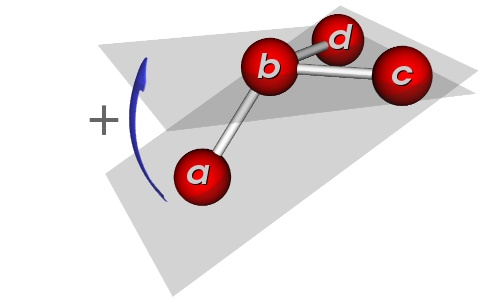
\includegraphics[width=7.5cm]{./Potentials/ImproperTorsionAnglePlus.jpg}
  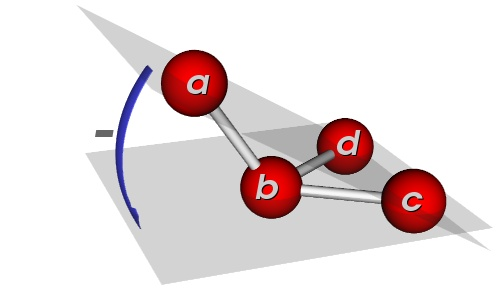
\includegraphics[width=7.5cm]{./Potentials/ImproperTorsionAngleMinus.jpg}
  \caption{The most common (CVFF, DLPOLY) definition of the improper dihedral angle 
   $\phi$: the angle between the planes formed by atoms `a-c-d' and `c-d-b'.
   On the left a positive improper dihedral angle, and on the right a negative improper dihedral angle.
   The atoms need to be listed in the order `a-c-d-b'. Note that an exchange of atoms `c' and `d' leads to a change
   of sign, but \emph{not} in magntitude.}
  \label{Fig: Improper Torsion definition}
  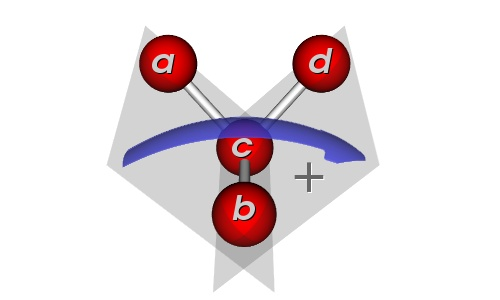
\includegraphics[width=7.5cm]{./Potentials/ImproperTorsionAngleTypeA.jpg}
  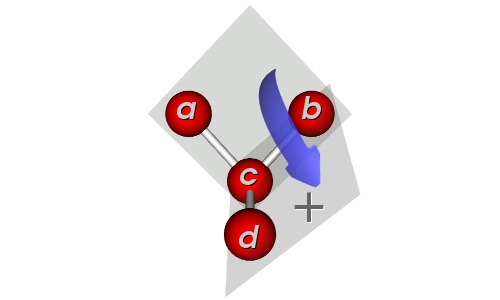
\includegraphics[width=7.5cm]{./Potentials/ImproperTorsionAngleTypeB.jpg}
  \caption{A second definition of the improper dihedral angle (CHARMM, AMBER). The central atom is `c', and the improper torsion
   is enter as `a-b-c-d'. Howevere, an exchange of terminal atoms leads to a change in magntitude and the improper torsion
   needs to be symmetrized by adding two additional improper torsions `b-d-c-a' and `d-a-c-b' and rescaling the force constant
   by a factor of $1/3$.}
\end{figure}

The improper torsion is an alternative for the out-of-plane angle, and a possible definition is
\begin{equation}
  U=\frac{1}{2} k \left(1-\cos 2\chi\right)
\end{equation}
It is termed `improper torsion' because it simply treats the four atoms in the plane as if they were
bonded in the same way as in a true torsional angle. Note that the definition include one central atom
which is listed as the second in $a-b-c-d$: $a$, $c$, and $d$ are bonded to the central atom $b$.
Improper torsions are often used to keep sp2 atoms planar and sp3 atoms in a tetrahedral geometry.

The CHARMM convention is to list the central atom first, while there are no rules how to order the other three atoms.
Hence, six possibilities exist for the definition of an improper torsion. The AMBER convention is that the out-of-plane
atom is listed in the third position and the order of the other atoms is determined alphabetically by atom type, and
by the atom number (i.e. the order in the molecule) when atom types are identical.

\begin{itemize}
  \item{HARMONIC\_IMPROPER\_DIHEDRAL}\\
  \begin{equation}
  U=\frac{1}{2}p_0\left(\phi_{ijkl}-p_1\right)^2
  \end{equation}
  2 arguments: $p_0/k_B$ in units of K/rad$^2$, $p_1$ in degrees.

  \item{HARMONIC\_COSINE\_IMPROPER\_DIHEDRAL}\\
  \begin{equation}
  U=\frac{1}{2}p_0\left[\cos\left(\phi_{ijkl}\right)-\cos\left(p_1\right)\right]^2
  \end{equation}
  2 arguments: $p_0/k_B$ in units of K, $p_1$ in degrees.

  \item{THREE\_COSINE\_IMPROPER\_DIHEDRAL}\\
  \begin{equation}
  U=\frac{1}{2}p_0\left[1+\cos\left(\phi_{ijkl}\right)\right]+
    \frac{1}{2}p_1\left[1-\cos\left(2\phi_{ijkl}\right)\right]+
    \frac{1}{2}p_2\left[1+\cos\left(3\phi_{ijkl}\right)\right]
  \end{equation}
  3 arguments: $p_0/k_B,p_1/k_B,p_2/k_B$ in units of K.

  \item{MM3\_IMPROPER\_DIHEDRAL}\\
  \begin{equation}
  U=\frac{1}{2}p_0\left[1+\cos\left(\phi_{ijkl}\right)\right]+
    \frac{1}{2}p_1\left[1-\cos\left(2\phi_{ijkl}\right)\right]+
    \frac{1}{2}p_2\left[1+\cos\left(3\phi_{ijkl}\right)\right]
  \end{equation}
  3 arguments: $p_0,p_1,p_2$ in units of kcal/mol.


  \item{CFF\_IMPROPER\_DIHEDRAL}\\
  \begin{equation}
  U=p_0\left[1-\cos\left(\phi_{ijkl}\right)\right]+
    p_1\left[1-\cos\left(2\phi_{ijkl}\right)\right]+
    p_2\left[1-\cos\left(3\phi_{ijkl}\right)\right]
  \end{equation}
  3 arguments: $p_0/k_B,p_1/k_B,p_2/k_B$ in units of K.

  \item{CFF\_IMPROPER\_DIHEDRAL2}\\
  \begin{equation}
  U=p_0\left[1+\cos\left(\phi_{ijkl}\right)\right]+
    p_1\left[1+\cos\left(2\phi_{ijkl}\right)\right]+
    p_2\left[1+\cos\left(3\phi_{ijkl}\right)\right]
  \end{equation}
  3 arguments: $p_0/k_B,p_1/k_B,p_2/k_B$ in units of K.

  \item{SIX\_COSINE\_IMPROPER\_DIHEDRAL}\\
  The Ryckaert-Bellemans potentials is often used for alkanes, the use implies exclusion of VDW-interactions
  between the first and last atoms of the dihedral, and $\phi'=\phi-\pi$ is defined according to the
  polymer convention $\phi'(trans)=0$.
  \begin{align}
  U=&\sum_{n=0}^5 p_n \cos^n\left(\phi'_{ijkl}\right)\\
    =&p_0+p_1\cos\left(\phi'_{ijkl}\right)+p_2\cos^2\left(\phi'_{ijkl}\right)+p_3\cos^3\left(\phi'_{ijkl}\right)
    p_4\cos^4\left(\phi'_{ijkl}\right)+p_5\cos^5\left(\phi'_{ijkl}\right)
  \end{align}
  6 arguments: $p_0/k_B,\dots,p_5/k_B$ in units of K.
  Rewritten in terms of $\phi$ the potential reads
  \begin{equation}
  U=p_0-p_1\cos\left(\phi_{ijkl}\right)+p_2\cos^2\left(\phi_{ijkl}\right)
    -p_3\cos^3\left(\phi_{ijkl}\right)+p_4\cos^4\left(\phi_{ijkl}\right)
    -p_5\cos^5\left(\phi_{ijkl}\right)
  \end{equation}

  \item{TRAPPE\_IMPROPER\_DIHEDRAL}\\
  \begin{equation}
  U=p_0+p_1\left[1+\cos\left(\phi_{ijkl}\right)\right]+
        p_2\left[1-\cos\left(2\phi_{ijkl}\right)\right]+
        p_3\left[1+\cos\left(3\phi_{ijkl}\right)\right]
  \end{equation}
  4 arguments: $p_0/k_B,p_1/k_B,p_2/k_B,p_3/k_B$ in units of K.

  \item{CVFF\_IMPROPER\_DIHEDRAL}\\
  \begin{equation}
  U=p_0\left[1+\cos\left(p_1\phi_{ijkl}-p_2\right)\right]
  \end{equation}
  3 arguments: $p_0/k_B$ in units of K, $p_1$ dimensionless, and $p_2$ in degrees.

  \item{OPLS\_IMPROPER\_DIHEDRAL}\\
  \begin{equation}
  U= \frac{1}{2}p_0+
    \frac{1}{2}p_1\left[1+\cos\left(\phi_{ijkl}\right)\right]+
    \frac{1}{2}p_2\left[1-\cos\left(2\phi_{ijkl}\right)\right]+
    \frac{1}{2}p_3\left[1+\cos\left(3\phi_{ijkl}\right)\right]
  \end{equation}
  4 arguments: $p_0/k_B,p_1/k_B,p_2/k_B,p_3/k_B$ in units of K.

  \item{FOURIER\_SERIES\_IMPROPER\_DIHEDRAL}\\
  The general form of a Fourier expansion is:
  \begin{equation}
  U=\sum_{n=1}^6\left[a_n\cos\left(n\phi\right)+b_n\sin\left(n\phi\right)\right]
  \end{equation}
  This form uses equilibrium angles of 0 for $n=1,3,5$ and 180 for $n=2,4,6$
  \begin{equation}
  \begin{split}
  U=&\frac{1}{2}p_0\left[1+\cos\phi\right]+
    \frac{1}{2}p_1\left[1-\cos\left(2\phi\right)\right]+
    \frac{1}{2}p_2\left[1+\cos\left(3\phi\right)\right]+\\
    &\frac{1}{2}p_3\left[1-\cos\left(4\phi\right)\right]+
    \frac{1}{2}p_4\left[1+\cos\left(5\phi\right)\right]+
    \frac{1}{2}p_5\left[1-\cos\left(6\phi\right)\right]
  \end{split}
  \end{equation}
  6 arguments: $p_0/k_B,p_1/k_B,p_2/k_B,p_3/k_B,p_4/k_B,p_5/k_B$ in units of K.

  \item{FOURIER\_SERIES\_IMPROPER\_DIHEDRAL\_2}\\  The general form of a Fourier expansion is:
  \begin{equation}
  U=\sum_{n=1}^6\left[a_n\cos\left(n\phi\right)+b_n\sin\left(n\phi\right)\right]
  \end{equation}
  This form uses equilibrium angles of 0 for $n=1,3,4,5,6$ and 180 for $n=2$
  \begin{equation}
  \begin{split}
  U=&\frac{1}{2}p_0\left[1+\cos\phi\right]+
    \frac{1}{2}p_1\left[1-\cos\left(2\phi\right)\right]+
    \frac{1}{2}p_2\left[1+\cos\left(3\phi\right)\right]+\\
    &\frac{1}{2}p_3\left[1+\cos\left(4\phi\right)\right]+
    \frac{1}{2}p_4\left[1+\cos\left(5\phi\right)\right]+
    \frac{1}{2}p_5\left[1+\cos\left(6\phi\right)\right]
  \end{split}
  \end{equation}
  6 arguments: $p_0/k_B,p_1/k_B,p_2/k_B,p_3/k_B,p_4/k_B,p_5/k_B$ in units of K.
  \item{FIXED\_IMPROPER\_DIHEDRAL}\\
   Use for improper-dihedral-angle constraint using the `SHAKE' and `RATTLE'-algorithm.      
   Applies to Molecular Dynamics and minimization. Does not work (yet) in Monte-Carlo.

\end{itemize}


\section{Non-bonded potentials}

\subsection{Van der Waals potentials}

The general expression for Van der Waals potentials when using a cutoff distance is
\begin{equation}
 U_{ij}^{\text{VDW}}=\begin{cases}
    U_{ij}\left(r_{ij}\right)& \text{if }r_{ij}\leq r_c\\
    0 & \text{otherwise}
   \end{cases}
\end{equation}

\begin{itemize}

  \item{NONE}\\
  \begin{equation}
    U=0
  \end{equation}
  zero parameters.
\item{$\begin{array}{l}\text{LENNARD\_JONES}\\
      \text{LENNARD\_JONES\_SMOOTHED3}\\
      \text{LENNARD\_JONES\_SMOOTHED5}\end{array}$}\\
  \begin{equation}
    U= 
      4 p_0 \left[\left(\frac{p_1}{r}\right)^{12}-\left(\frac{p_1}{r}\right)^6\right]
  \end{equation}
  2 parameters: $p_0/k_B$ in units of K, and $p_1$ in \AA.
\item{$\begin{array}{l}\text{FEYNMAN\_HIBBS\_LENNARD\_JONES}\\
      \text{FEYNMAN\_HIBBS\_LENNARD\_JONES\_SMOOTHED3}\\
      \text{FEYNMAN\_HIBBS\_LENNARD\_JONES\_SMOOTHED5}\end{array}$}\\
  \begin{equation}
    U=4 p_0 \left[\left(\frac{p_1}{r}\right)^{12}-\left(\frac{p_1}{r}\right)^6\right]
      +\frac{\hbar^2}{24 p_2 k_B T} 4 p_0\left[132\left(\frac{p_1}{r}\right)^{12}-30\left(\frac{p_1}{r}\right)^6\right]\frac{1}{r^2}
  \end{equation}
  3 parameters: $p_0/k_B$ in units of K, $p_1$ in \AA, and $p_2$ is the reduced mass in unified atomic mass units.

\item{$\begin{array}{l}\text{FEYNMAN\_HIBBS2\_LENNARD\_JONES}\\
      \text{FEYNMAN\_HIBBS\_LENNARD\_JONES2\_SMOOTHED3}\\
      \text{FEYNMAN\_HIBBS\_LENNARD\_JONES2\_SMOOTHED5}\end{array}$}\\
  \begin{equation}
    U=4 p_0 \left[\left(\frac{p_1}{r}\right)^{12}-\left(\frac{p_1}{r}\right)^6\right]
      +4 p_0\left[132\left(\frac{p_1}{r}\right)^{12}-30\left(\frac{p_1}{r}\right)^6\right]\frac{p_2}{r^2}
  \end{equation}
  3 parameters: $p_0/k_B$ in units of K, $p_1$ in \AA, and $p_2$ in units of $\AA^2$.

  \item{LENNARD\_JONES\_SHIFTED\_FORCE}\\
  \begin{equation}
       U=4 p_0 \left\{\left[\left(\frac{p_1}{r}\right)^{12}-\left(\frac{p_1}{r}\right)^6\right]-
           \left[\left(\frac{p_1}{r_c}\right)^{12}-\left(\frac{p_1}{r_c}\right)^6\right]+
           \left[12\left(\frac{p_1}{r_c}\right)^{12}-6\left(\frac{p_1}{r_c}\right)^{6}\right]\frac{\left(r-r_c\right)}{r_c}\right\}
  \end{equation}
  2 parameters: $p_0/k_B$ in units of K, and $p_1$ in \AA.

  \item{LENNARD\_JONES\_SHIFTED\_FORCE2}\\
  \begin{equation}
       4 p_0 \left\{\left[\left(\frac{p_1}{r}\right)^{12}-\left(\frac{p_1}{r}\right)^6\right]
       +\left[6\left(\frac{p_1}{r_c}\right)^{12}-3\left(\frac{p_1}{r_c}\right)^6\right]\frac{r^2}{r_c^2}
       +7\left(\frac{p_1}{r_c}\right)^{12}+4\left(\frac{p_1}{r_c}\right)^6\right\}
  \end{equation}
  2 parameters: $p_0/k_B$ in units of K, and $p_1$ in \AA.

\item{$\begin{array}{l}\text{POTENTIAL\_12\_6}\\
      \text{POTENTIAL\_12\_6\_SMOOTHED3}\\
      \text{POTENTIAL\_12\_6\_SMOOTHED5}\end{array}$}\\
  \begin{equation}
    U= 
      \frac{p_0}{r^{12}}-\frac{p_1}{r^6}
  \end{equation}
   2 parameters: $p_0/k_B$ in units of K\,\AA$^{12}$, and $p_1/k_B$ in units of K\,\AA$^6$.

\item{$\begin{array}{l}\text{POTENTIAL\_12\_6\_2\_0}\\
      \text{POTENTIAL\_12\_6\_2\_0\_SMOOTHED3}\\
      \text{POTENTIAL\_12\_6\_2\_0\_SMOOTHED5}\end{array}$}\\
  \begin{equation}
    U= 
      \frac{p_0}{r^{12}}+\frac{p_1}{r^6}+\frac{p_2}{r^2}+p_3
  \end{equation}
   4 parameters: $p_0/k_B$ in units of K\,\AA$^{12}$, $p_1/k_B$ in units of K\,\AA$^6$, $p_2/k_B$ in units of K\,\AA$^2$, 
   and $p_3$ in units of K.

\item{$\begin{array}{l}\text{MORSE}\\
      \text{MORSE\_SMOOTHED3}\\
      \text{MORSE\_SMOOTHED5}\end{array}$}\\
  \begin{equation}
    U= p_0 \left[(1-{e^{-p_1*(r-p_2)}})^2-1\right]
  \end{equation}
   3 parameters: $p_0/k_B$ in units of K, $p_1$ in units of $\AA^{-1}$ and $p_2$ in units of \AA.

\item{$\begin{array}{l}\text{MORSE2}\\
      \text{MORSE2\_SMOOTHED3}\\
      \text{MORSE2\_SMOOTHED5}\end{array}$}\\
  \begin{equation}
    U= p_0 \left[e^{p_1*(1-r/p_2)}-2e^{(p_1/2)*(1-r/p_2)}\right]
  \end{equation}
   3 parameters: $p_0/k_B$ in units of K, $p_1$ in units of $\AA^{-1}$ and $p_2$ in units of \AA.

\item{$\begin{array}{l}\text{MORSE3}\\
      \text{MORSE3\_SMOOTHED3}\\
      \text{MORSE3\_SMOOTHED5}\end{array}$}\\
  \begin{equation}
    U= p_0 \left[\left(1-e^{\left(\frac{-\ln{2}}{2^{\nicefrac{1}{6}}-1}\right)\left(\frac{r}{p_2}-2^{\nicefrac{1}{6}}\right)}\right)^2-1\right]
  \end{equation}
   2 parameters: $p_0/k_B$ in units of K $p_2$ in units of \AA. This form of the Morse potential resembles the Lennard-Jones potential.

\item{$\begin{array}{l}\text{CFF\_9\_6}\\
      \text{CFF\_9\_6\_SMOOTHED3}\\
      \text{CFF\_9\_6\_SMOOTHED5}\end{array}$}\\
  \begin{equation}
    U= 
      \frac{p_0}{r^{9}}-\frac{p_1}{r^6}
  \end{equation}
   2 parameters: $p_0/k_B$ in units of K\,\AA$^{9}$, and $p_1/k_B$ in units of K\,\AA$^6$.

\item{$\begin{array}{l}\text{CFF\_EPS\_SIGMA}\\
      \text{CFF\_EPS\_SIGMA\_SMOOTHED3}\\
      \text{CFF\_EPS\_SIGMA\_SMOOTHED5}\end{array}$}\\
  \begin{equation}
    U_{ij}= 
      p_0 \left[2\left(\frac{p_1}{r}\right)^{9}-3\left(\frac{p_1}{r}\right)^6\right]
  \end{equation}
  2 parameters: $p_0/k_B$ in units of K, and $p_1$ in \AA.

\item{$\begin{array}{l}\text{BUCKINGHAM}\\
      \text{BUCKINGHAM\_SMOOTHED3}\\
      \text{BUCKINGHAM\_SMOOTHED5}\end{array}$}\\
  \begin{equation}
  U=
     p_0 e^{-p_1 r}-\frac{p_2}{r^{6}}
  \end{equation}
  3 parameters: $p_0/k_B$ in units of K, $p_1$ in units of \AA$^{-1}$, and $p_2$ in K\,\AA$^6$. Warning: in literature sometimes $\rho=\frac{1}{p_1}$ is given,
  $\rho$ is usually around 0.3-0.4 \AA, $p_1$ is usually around 2-4 \AA$^{-1}$.

\item{$\begin{array}{l}\text{BUCKINGHAM2}\\
      \text{BUCKINGHAM2\_SMOOTHED3}\\
      \text{BUCKINGHAM2\_SMOOTHED5}\end{array}$}\\
  \begin{equation}
  U=\begin{cases}
     10^{10}  & r<p_3\\
     p_0 e^{-p_1 r}-\frac{p_2}{r^{6}} & \text{otherwise}
    \end{cases}
  \end{equation}
  4 parameters: $p_0/k_B$ in units of K, $p_1$ in units of \AA$^{-1}$, $p_2$ in K\,\AA$^6$, and $p_3$ in [\AA].
  Warning: in literature sometimes $\rho=\frac{1}{p_1}$ is given,
  $\rho$ is usually around 0.3-0.4 \AA, $p_1$ is usually around 2-4 \AA$^{-1}$.

\item{$\begin{array}{l}\text{MM3\_VDW}\\
      \text{MM3\_VDW\_SMOOTHED3}\\
      \text{MM3\_VDW\_SMOOTHED5}\end{array}$}\\
  \begin{equation}
    U_{ij}= \begin{cases}
       \sqrt{p_0^i p_0^j}\left[1.84\times10^5 e^{-\frac{12}{P}}-2.25\,P^6\right] & \text{if }P\geq 3.02\\
       \sqrt{p_0^i p_0^j} 192.27 P^2  & \text{if }P<3.02
       \end{cases}
  \end{equation}
  with $P=\frac{p_1^i+p_1^j}{r_{ij}}$ and where $p_1^i$ and $p_1^j$ are the VDW radii of atoms $i$ and $j$,
  and $r_{ij}$ the separation distance in \AA\ between atoms $i$ and $j$. \\
  2 arguments: $p_0$ in units of kcal/mol, $p_1$ in units of \AA.

\item{$\begin{array}{l}\text{MATSUOKA\_CLEMENTI\_YOSHIMINE}\\
      \text{MATSUOKA\_CLEMENTI\_YOSHIMINE\_SMOOTHED3}\\
      \text{MATSUOKA\_CLEMENTI\_YOSHIMINE\_SMOOTHED5}\end{array}$}\\
  \begin{equation}
    U= p_0e^{-p_1 r_{ij}}+p_2e^{-p_3 r_{ij}}
  \end{equation}
   4 arguments: $p_0/k_B$ in units of K, $p_1$ in units of \AA$^{-1}$, $p_2/k_B$ in units of K, and $p_3$ in units of \AA$^{-1}$.

\item{$\begin{array}{l}\text{GENERIC}\\
      \text{GENERIC\_SMOOTHED3}\\
      \text{GENERIC\_SMOOTHED5}\end{array}$}\\
  \begin{equation}
    U= p_0 e^{-p_1 r}-\frac{p_2}{r^4}-\frac{p_3}{r^6}-\frac{p_4}{r^8}-\frac{p_5}{r^{10}}
  \end{equation}
  6 arguments: $p_0/k_B$ in units of K, $p_1$ in units of \AA$^{-1}$, $p_2/k_B$ in units of K\,\AA$^{4}$, $p_3/k_B$ in units of K\,\AA$^{6}$,
  $p_4/k_B$ in units of K\,\AA$^{8}$, and $p_5/k_B$ in units of K\,\AA$^{10}$.

\item{$\begin{array}{l}\text{PELLENQ\_NICHOLSON}\\
      \text{PELLENQ\_NICHOLSON\_SMOOTHED3}\\
      \text{PELLENQ\_NICHOLSON\_SMOOTHED5}\end{array}$}\\
  \begin{equation}
    U= p_0 e^{-p_1 r}-f_6 \frac{p_2}{r^6}-f_8\frac{p_3}{r^8}-f_{10}\frac{p_4}{r^{10}}
  \end{equation}
  with
  \begin{equation}
   f_{2n}=1-\sum_{k=0}^{2n}\frac{\left(p_1 r_{ij}\right)^k}{k!} e^{-p_1 r_{ij}}
  \end{equation}
  5 arguments: $p_0/k_B$ in units of K, $p_1$ in units of \AA$^{-1}$, $p_2/k_B$ in units of K\,\AA$^{6}$,
  $p_3/k_B$ in units of K\,\AA$^{8}$, and $p_4/k_B$ in units of K\,\AA$^{10}$.

\item{$\begin{array}{l}\text{HYDRATED\_ION\_WATER}\\
      \text{HYDRATED\_ION\_WATER\_SMOOTHED3}\\
      \text{HYDRATED\_ION\_WATER\_SMOOTHED5}\end{array}$}\\
  \begin{equation}
    U= p_0 e^{-p_1 r}-\frac{p_2}{r^4}-\frac{p_3}{r^6}-\frac{p_4}{r^{12}}
  \end{equation}
  5 arguments: $p_0/k_B$ in units of K, $p_1$ in units of \AA$^{-1}$, $p_2/k_B$ in units of K\,\AA$^{4}$,
  $p_3/k_B$ in units of K\,\AA$^{6}$, and $p_4/k_B$ in units of K\,\AA$^{12}$.

\item{$\begin{array}{l}\text{MIE}\\
      \text{MIE\_SMOOTHED3}\\
      \text{MIE\_SMOOTHED5}\end{array}$}\\
The Mie-potential \cite{Mie1903}
  \begin{equation}
    U= 
      \left(\frac{p_0}{r^{p_1}}-\frac{p_2}{r^{p_3}}\right)
  \end{equation}
   4 arguments: $p_0/k_B$ in units of K \AA$^{p_1}$, $p_1$ dimensionless,
  $p_2/k_B$ in units of K \AA$^{p_3}$, and $p_3$ dimensionless.

\item{$\begin{array}{l}\text{BORN\_HUGGINS\_MEYER}\\
      \text{BORN\_HUGGINS\_MEYER\_SMOOTHED3}\\
      \text{BORN\_HUGGINS\_MEYER\_SMOOTHED5}\end{array}$}\\
  \begin{equation}
    U_{ij}=p_0 e^{p_1\left(p_2-r_{ij}\right)}-\frac{p_3}{r_{ij}^6}-\frac{p_4}{r_{ij}^8}
  \end{equation}
  5 arguments: $p_0/k_B$ in units of K, $p_1$ dimensionless, $p_2$ in units of \AA, $p_3/k_B$ in units of K\,\AA$^{6}$, and
  $p_4/k_B$ in units of K\,\AA$^{8}$.

\item{$\begin{array}{l}\text{HYDROGEN}\\
      \text{HYDROGEN\_SMOOTHED3}\\
      \text{HYDROGEN\_SMOOTHED5}\end{array}$}\\
  \begin{equation}
    U= 
      \frac{p_0}{r^{12}}-\frac{p_1}{r^{10}}
  \end{equation}
   2 arguments: $p_0/k_B$ in units of K\,\AA$^{12}$, and $p_1/k_B$ in units of K\,\AA$^{10}$.

\end{itemize}

\subsection{Tail corrections}

\subsubsection*{energy}

\begin{equation}
 U^{\text{Tail}}=\frac{2 \pi}{V}\sum_a \sum_b N_a N_b \left[\int_{r_c}^\infty r^2 U\left(r\right)\, dr\right]
\end{equation}

\begin{tabular}{|l|l|}
\hline
potential & $\int_{r_c}^\infty r^2 U\left(r\right)$\\
\hline\hline
  LENNARD\_JONES &
      $\frac{4}{3}\,p_0\,p_1^3 \left[\frac{1}{3}\left(\frac{p_1}{r}\right)^{9}-\left(\frac{p_1}{r}\right)^3\right]$\\
  LENNARD\_JONES\_SHIFTED\_FORCE & -\\
\hline
\end{tabular}

\subsubsection*{pressure}
\begin{align}
 P^{\text{Tail}}=&-\sum_a \sum_b \frac{2\pi}{3V} N_a N_b \left[\int_{r_c}^\infty r^2\, r\frac{\partial U\left(r\right)}{\partial r}\, dr\right]\\
    =&\sum_a \sum_b\left(\frac{2\pi}{3V} r_c^3 N_a N_b U\left(r_c\right)+U^{\text{Tail}}\right)
\end{align}
\subsubsection*{chemical potential}
\begin{equation}
 \beta \mu^{\text{Tail}}=2 U^{\text{Tail}}
\end{equation}

\subsection{Electrostatics}

\subsubsection{Charge-charge interaction}
\begin{itemize}
\item{Ewald}\\
The potential energy for a system of charges in a periodic system can be written as
\begin{equation}
 U=U^{\text{real}}+U^{\text{rec}}
\end{equation}
where
\begin{equation}
 \begin{split}
 U^{\text{real}}
  &=\sum_{i<j} q_i q_j \frac{\text{erfc}\left(\alpha r_{ij}\right)}{r_{ij}}\\
 U^{\text{rec}}
  &=\frac{2\pi}{V}\sum_{\mathbf{k}\not=0}\frac{1}{k^2} e^{-\frac{k^2}{4\alpha^2}}
  \left(\left|\sum_{i=1}^N q_i\cos\left(\mathbf{k}\cdot\mathbf{r}_i\right)\right|^2+
   \left|\sum_{i=1}^N q_i\sin\left(\mathbf{k}\cdot\mathbf{r}_i\right)\right|^2\right)
 -\sum_i\frac{\alpha}{\sqrt{\pi}}q_i^2
 \end{split}
\end{equation}
where $q_i$ and $q_j$ are the charges of particle $i$ and $j$, respectively, $\mathbf{r}_i$ the position of atom $i$, $V$ the volume of the cell,
$\alpha$ a damping factor, $k$ the wavelength, and `erfc' the error function complement. The expression gives the \emph{exact} solution for charges
in a periodic system up to arbitrary precision. One part is computed in `real' space, and the long-range part is more conveniently computed in Fourier space.

\item{CoulombTruncated}
\begin{equation}
 U=\begin{cases}
    \sum_{i<j} \frac{1}{4\pi\epsilon}\frac{q_i q_j}{r_{ij}}& \text{if }r_{ij}\leq r_c\\
    0 & \text{otherwise}
   \end{cases}
\end{equation}

\item{CoulombShifted}
\begin{equation}
 U=\begin{cases}
    \sum_{i<j} \frac{q_i q_j}{4\pi \epsilon }\left(\frac{1}{r_{ij}}-\frac{1}{r_c}\right)& \text{if }r_{ij}\leq r_c\\
    0 & \text{otherwise}
   \end{cases}
\end{equation}

\item{CoulombSmoothed}
\item{Wolf}

\end{itemize}

\subsubsection{Charge-dipole interaction}

\begin{itemize}
\item{Ewald}\\
\item{CoulombTruncated}
\begin{equation}
 U=\begin{cases}
    \sum_{i,j} \frac{1}{4\pi\epsilon} \frac{-q_i}{r^2_{ij}}
      \left({\boldsymbol \mu}_j\cdot\mathbf{r}_{ij}\right)& \text{if }r_{ij}\leq r_c\\
    0 & \text{otherwise}
   \end{cases}
\end{equation}
\end{itemize}


\subsubsection{Dipole-dipole interaction}

\begin{itemize}
\item{Ewald}\\
\item{CoulombTruncated}
\begin{equation}
 U=\begin{cases}
    \sum_{i,j} \frac{1}{4\pi\epsilon}\frac{1}{r^3_{ij}}
    \left[{\boldsymbol \mu}_i\cdot {\boldsymbol \mu}_j-3\frac{\left({\boldsymbol\mu}_i\cdot\mathbf{r}_{ij}\right)
    \left(\mathbf{r}_{ij}\cdot{\boldsymbol \mu}_j\right)}{r^2_{ij}}\right]& \text{if }r_{ij}\leq r_c\\
    0 & \text{otherwise}
   \end{cases}
\end{equation}
\end{itemize}


\section{Bonded potentials cross terms}

\subsection{Bond-bond potential}

\begin{itemize}
  \item{CFF\_BOND\_BOND\_CROSS,CVFF\_BOND\_BOND\_CROSS}\\
  \begin{equation}
  U=p_0\left(r-p_1\right)\left(r'-p_2\right)
  \end{equation}
  3 arguments: $p_0/k_B$ in units of K/\AA$^2$, $p_0$ and $p_1$ in \AA.
\end{itemize}

\subsection{Bond-bend potential}

\begin{itemize}
  \item{CFF\_BOND\_BEND\_CROSS,CVFF\_BOND\_BEND\_CROSS}\\
  \begin{equation}
  U=\left(\theta-p_0\right)\left[p_1\left(r-p_2\right)+p_3\left(r'-p_4\right)\right]
  \end{equation}
  5 arguments: $p_0$ in degrees, $p_1/k_B$ in units of K/\AA/rad, $p_2$ in \AA, $p_3/k_B$ in units of K/\AA/rad, $p_4$ in \AA.

  \item{MM3\_BOND\_BEND\_CROSS}
  \begin{equation}
  U=p_0\left[\left(r-p_1\right)+\left(r'-p_2\right)\right]\left(\theta-p_3\right)
  \end{equation}
  4 arguments: $p_0$ in mdyne/rad, $p_1$ and $p_2$ in \AA, and $p_3$ in degrees.

  \item{TRUNCATED\_HARMONIC}
  \begin{equation}
  U=\frac{1}{2}p_0\left(\theta-p_1\right)^2 e^{-\frac{r_{ij}^8+r_{ik}^8}{p_2^8}}
  \end{equation}
  3 arguments: $p_0/k_B$ in K/rad$^2$, $p_1$ in degrees, and $p_2$ in units of \AA.

  \item{SCREENED\_HARMONIC}
  \begin{equation}
  U=\frac{1}{2}p_0\left(\theta-p_1\right)^2 e^{-\left(\frac{r_{ij}}{p_2}+\frac{r_{ik}}{p_3}\right)}
  \end{equation}
  4 arguments: $p_0$ in K/rad$^2$, $p_1$ in degrees, $p_2$ and $p_3$ in units of \AA.

  \item{SCREENED\_VESSAL}
  \begin{equation}
  U=\frac{p_0}{8\left(\theta_{ijk}-\pi\right)^2}
    \left[\left(p_1-\pi\right)^2-\left(\theta_{ijk}-\pi\right)^2\right]^2
    e^{-\left(\frac{r_{ij}}{p_2}+\frac{r_{ik}}{p_3}\right)}
  \end{equation}
  4 arguments: $p_0$ in K/rad$^2$, $p_1$ in degrees, $p_2$ and $p_3$ in units of \AA.

  \item{TRUNCATED\_VESSAL}
  \begin{equation}
  U=p_0\left[
   \theta_{ijk}^{p_2}\left(\theta_{ijk}-p_1\right)^2
     \left(\theta_{ijk}+p_1-2\pi\right)^2-\frac{p_2}{2}\pi^{p_2-1}
      \left(\theta_{ijk}-p_1\right)^2\left(\pi-p_1\right)^3
    e^{-\frac{r_{ij}^8+r_{ik}^8}{p_3^8}}
    \right]
  \end{equation}
  4 arguments: $p_0$ in K/rad$^{4+p_2}$, $p_1$ in degrees, $p_2$ dimensionless, and $p_3$ in \AA.

\end{itemize}

\subsection{Bend-bend potential}

\begin{itemize}
  \item{CFF\_BEND\_BEND\_CROSS,CVFF\_BEND\_BEND\_CROSS}\\
  \begin{equation}
  U=p_0\left(\theta-p_1\right)\left(\theta'-p_2\right)
  \end{equation}
  3 arguments: $p_0$ in units of K/rad$^2$, $p_1$ and $p_2$ in units of degrees.

 \item{MM3\_BEND\_BEND\_CROSS}
  \begin{equation}
  U=-p_0\left(\theta-p_1\right)\left(\theta'-p_2\right)
  \end{equation}
  3 arguments: $p_0$ in units of mdyne/rad$^2$, $p_1$ and $p_2$ in units of degrees.
\end{itemize}

\subsection{Bond-torsion potential}

The bond-torsions potential correlates the torsion $i-j-k-l$ with the central bond $j-k$,
or with the two terminating bonds.

\begin{itemize}
 \item{MM3\_BOND\_TORSION\_CROSS}\\
The MM3 bond-torsion potential correlates the torsion $i-j-k-l$ with the central bond $j-k$
  \begin{equation}
  U=\frac{1}{2}p_0\left(r-p_3\right)\left(1+\cos\phi\right)+
    \frac{1}{2}p_1\left(r-p_3\right)\left(1+\cos2\phi\right)+
    \frac{1}{2}p_2\left(r-p_3\right)\left(1+\cos3\phi\right)
  \end{equation}
  4 arguments: $p_0,p_1,p_2$ in units of kcal/mol, $p_3$ the reference length of the central bond in \AA.
\end{itemize}


\subsection{Bend-torsion potential}

\begin{itemize}
  \item{CFF\_BEND\_TORSION\_CROSS,CVFF\_BEND\_TORSION\_CROSS}\\
  \begin{equation}
  U=p_0\left(\theta-p_1\right)\left(\theta'-p_2\right)\cos\phi
  \end{equation}
  3 arguments: $p_0$ in units of K/rad$^3$, $p_1$ and $p_2$ in units of degrees.
\item{SMOOTHED\_DIHEDRAL}
  \begin{equation}
  U=p_0\left(1+\cos(p_1\phi_{ijkl}-p_2\right)S\left(\theta_{ijk}\right)S\left(\theta_{jkl}\right)
  \end{equation}
  3 arguments: $p_0/k_B$ in units of K/rad$^2$, $p_1$ dimensionless, and  $p_2$ in degrees.

\item{SMOOTHED\_THREE\_COSINE\_DIHEDRAL}
  \begin{equation}
  U=\left\{\frac{1}{2}p_0\left[1+\cos\left(\phi_{ijkl}\right)\right]+
    \frac{1}{2}p_1\left[1-\cos\left(2\phi_{ijkl}\right)\right]+
    \frac{1}{2}p_2\left[1+\cos\left(3\phi_{ijkl}\right)\right]\right\}
    S\left(\theta_{ijk}\right)S\left(\theta_{jkl}\right)
  \end{equation}
  3 arguments: $p_0/k_B,p_1/k_B,p_2/k_B$ in units of K.

\item{SMOOTHED\_CFF\_DIHEDRAL}
  \begin{equation}
  U=\left\{p_0\left[1-\cos\left(\phi_{ijkl}\right)\right]+
    p_1\left[1-\cos\left(2\phi_{ijkl}\right)\right]+
    p_2\left[1-\cos\left(3\phi_{ijkl}\right)\right]\right\}
    S\left(\theta_{ijk}\right)S\left(\theta_{jkl}\right)
  \end{equation}
  3 arguments: $p_0/k_B,p_1/k_B,p_2/k_B$ in units of K.

\item{SMOOTHED\_CFF\_DIHEDRAL2}
  \begin{equation}
  U=\left\{p_0\left[1+\cos\left(\phi_{ijkl}\right)\right]+
    p_1\left[1+\cos\left(2\phi_{ijkl}\right)\right]+
    p_2\left[1+\cos\left(3\phi_{ijkl}\right)\right]\right\}
    S\left(\theta_{ijk}\right)S\left(\theta_{jkl}\right)
  \end{equation}
  3 arguments: $p_0/k_B,p_1/k_B,p_2/k_B$ in units of K/rad.

\item{NICHOLAS\_DIHEDRAL}
 \begin{equation}
  U=\left\{\frac{1}{2}p_0\left[1+\cos\left(\phi_{ijkl}\right)\right]+
    \frac{1}{2}p_1\left[1-\cos\left(2\phi_{ijkl}\right)\right]+
    \frac{1}{2}p_2\left[1+\cos\left(3\phi_{ijkl}\right)\right]\right\}
    S\left(\theta_{ijk}\right)
  \end{equation}
  3 arguments: $p_0/k_B,p_1/k_B,p_2/k_B$ in units of K/rad.

\item{SMOOTHED\_CFF\_BEND\_TORSION\_CROSS}

\begin{equation}
 U=S\left(\theta_1\right) 
 \left[
 p_0*(Theta_1-p_1)*(\theta_2-p_2)\cos(\phi)
\right]
S\left(\theta_2\right)
\end{equation}
  3 arguments: $p_0/k_B$ in units K/rad$^3$, $p_1$ and $p_2$ in units of degrees.
\end{itemize}


\noindent The smoothing function $S\left(\theta\right)$ is defined as
\begin{equation}
 S\left(\theta\right)=\begin{cases}
  1 & \theta<\theta_{\text{on}}\\
  \left(\theta_{\text{off}}-\theta\right)^2 
       \frac{\theta_{\text{off}}+2\theta-3\theta_{\text{on}}}
       {\left(\theta_{\text{off}}-\theta_{\text{on}}\right)^3}& \theta\geq\theta_{\text{on}}
  \end{cases}
\end{equation}
with $\theta_{\text{on}}=170^\circ$ and $\theta_{\text{off}}=180^\circ$.


\bibliographystyle{unsrt}
\bibliography{Potentials/biblio}

